\documentclass[11pt]{article}

\usepackage[review]{acl}
\usepackage{times}
\usepackage{latexsym}
\usepackage[T1]{fontenc}
\usepackage[utf8]{inputenc}
\usepackage{microtype}
\usepackage{inconsolata}
\usepackage{booktabs}
\usepackage{multirow}
\usepackage{amsmath}
\usepackage{graphicx}
\usepackage{float}
\usepackage{url}
\usepackage{hyperref}

\newcommand{\yesprob}{p_{\mathrm{yes}}}

\title{Evaluating the Explanatory Validity of Structured LLM Rationales for Forecasting}
\author{Anonymous ACL submission}
\date{}

\begin{document}
\maketitle

\begin{abstract}
Accurate forecasting requires models to provide not only well-calibrated probabilities, but also explanations that make their reasoning inspectable under temporal uncertainty.
We study whether structured rationale prompts improve the forecasting behavior and explanatory quality of large language models (LLMs) on binary future-event questions.
We build a reproducible evaluation pipeline over 1,580 resolved Metaculus-style forecasting questions paired with resolution criteria and news evidence, and compare a neutral baseline against eight rationale structures: predicted event, key attribute, reasoning type, credibility, key conditions, step-by-step reasoning, uncertainty language, and temporal anchors.
Across Qwen2.5-7B-Instruct, Qwen3-32B, and GPT-OSS-120B, we evaluate accuracy, Brier score, expected calibration error, and rationale quality under two automatic LLM judges.
Our results show that structured rationales do not uniformly improve forecasting: temporal anchors and credibility framing can improve some models, while uncertainty-language and key-condition prompts often degrade calibration or accuracy.
Automatic rationale scores correlate with forecast correctness, with completeness and plausibility emerging as the strongest predictors in a SHAP analysis.
These findings suggest that rationale structure is a consequential design choice, but its benefits depend on the target model and evaluation objective.
\end{abstract}

\section{Introduction}

Forecasting future events informs decisions in policy, finance, public health, and strategic planning.
Large language models (LLMs) are increasingly used to generate forecasts accompanied by natural-language rationales, making them attractive for settings where users need both a probability and an explanation.
Yet this combination raises a central question: \textit{does changing the structure of an LLM's rationale improve the reliability of its forecast, or merely change the surface form of its explanation?}

This question matters because probabilistic forecasting is not evaluated only by whether a model chooses the correct label.
A useful forecaster should also be calibrated: events assigned high confidence should occur more often than events assigned low confidence.
At the same time, a rationale should make the forecast inspectable by identifying the relevant event, evidence, assumptions, uncertainty, and temporal constraints.
These goals need not coincide.
A detailed rationale can support an overconfident or incorrect prediction, while a comparatively terse rationale can accompany a well-calibrated forecast.
For forecasting systems, explanation quality and probabilistic reliability therefore have to be measured jointly rather than assumed to improve together.

\paragraph{Challenges in LLM Forecasting.}
Future-event forecasting is difficult for LLMs because it requires reasoning over incomplete evidence, changing temporal context, and verifiable outcomes that may occur after the evidence was written.
Models can overfit to salient evidence, miss resolution-relevant dates, conflate stated plans with realized outcomes, or express verbal uncertainty that is not aligned with numeric confidence.
Moreover, generated rationales may be post-hoc justifications: they can sound coherent without faithfully reflecting the computation that produced the forecast.
This makes forecasting a useful testbed for studying rationale validity, because every prediction can be externally scored after resolution.

\paragraph{Motivation.}
Our approach is motivated by two complementary literatures.
Research on judgmental and crowd forecasting shows that decomposing a question into assumptions, evidence, time horizons, and uncertainty can improve human forecasts \cite{tetlock2015superforecasting}.
More directly, prior work on forecast summarization proposes representing future-related statements through atomic components such as the predicted event, event attributes, source credibility, conditions, rationale, modality, and timestamp \cite{saha2025wisdom}.
Interpretability research, however, cautions that natural-language explanations should not be equated with faithful reasoning traces \cite{jacovi2020towards}.
We use these components as inspiration for our structured rationale variants and treat rationale structure as an experimental intervention: if a component such as temporal anchoring or key-condition enumeration helps LLM forecasting, this should be visible in accuracy, Brier score, calibration, or independently judged rationale quality.

\paragraph{Our Work.}
We evaluate structured LLM rationales on 1,580 resolved Metaculus-style binary forecasting questions paired with descriptions, resolution criteria, temporal metadata, and retrieved news evidence.
We compare a neutral baseline prompt with eight structured variants targeting predicted event restatement, key attribute specification, reasoning type declaration, source credibility, key conditions, step-by-step reasoning, uncertainty language, and temporal anchors.
For the complete checked-in sweep, we evaluate three target models---Qwen2.5-7B-Instruct, Qwen3-32B, and GPT-OSS-120B---across six temperature settings.
We score forecasts using accuracy, Brier score, and expected calibration error (ECE), and we evaluate rationale quality using two automatic LLM judges that rate plausibility, completeness, source consistency, non-hallucination, informativeness, and conciseness.
Finally, we use a SHAP-based diagnostic analysis to test which judged rationale attributes are most predictive of forecast correctness.

Our results show that rationale structure is consequential but not uniformly beneficial.
Temporal anchors yield the best mean Brier score for GPT-OSS-120B and slightly improve over its neutral baseline.
Credibility framing gives Qwen3-32B its best accuracy and ECE, although not its best Brier score.
For Qwen2.5-7B-Instruct, the neutral baseline remains strongest under accuracy and Brier score, suggesting that smaller or less robust models may not benefit from additional rationale constraints.
Across automatic rationale evaluations, completeness and plausibility are the strongest predictors of forecast correctness, while conciseness contributes little because most generated rationales already satisfy the requested length constraints.

\subsection{Research Questions}

We organize the study around three research questions:

\begin{itemize}
    \item \textbf{RQ1:} How do structured rationale components affect probabilistic forecasting performance, as measured by accuracy, Brier score, and ECE?
    \item \textbf{RQ2:} How do structured rationale components affect judged explanatory quality, including plausibility, completeness, source consistency, non-hallucination, informativeness, and conciseness?
    \item \textbf{RQ3:} Which judged rationale attributes are most associated with forecast correctness?
\end{itemize}

\subsection{Hypotheses}

Inspired by the future-related statement components discussed in forecast-summarization research \cite{saha2025wisdom}, we test eight component-level hypotheses corresponding to the eight structured rationale variants beyond the neutral baseline:

\begin{itemize}
    \item \textbf{H1: Predicted event.} Explicitly restating the predicted event improves alignment between the forecast, the resolution criterion, and the generated rationale.
    \item \textbf{H2: Key attribute.} Identifying the key attribute improves specificity by focusing the rationale on the decisive time, quantity, or actor.
    \item \textbf{H3: Reasoning type.} Declaring the reasoning type exposes systematic differences among speculative, plan-based, expert-forecast-based, and trend-based forecasts.
    \item \textbf{H4: Credibility.} Focusing on source credibility improves evidence grounding and reduces unsupported or weakly supported claims.
    \item \textbf{H5: Key conditions.} Enumerating key conditions improves causal precision by making the assumptions behind the forecast explicit.
    \item \textbf{H6: Step-by-step reasoning.} Step-by-step reasoning improves transparency, but may also introduce redundant or formulaic rationales.
    \item \textbf{H7: Uncertainty language.} Explicit uncertainty language improves perceived interpretability and may improve alignment between verbal uncertainty and numeric confidence.
    \item \textbf{H8: Temporal anchors.} Temporal anchors improve temporal grounding by making resolution-relevant dates and time ranges explicit.
\end{itemize}

\subsection{Contributions}

This work makes four contributions:

\begin{itemize}
    \item We introduce a reproducible framework for evaluating structured LLM rationales on resolved binary forecasting questions with evidence, resolution criteria, and temporal metadata.
    \item We provide a controlled comparison of a neutral forecasting prompt and eight structured rationale prompts across three fully evaluated LLMs and six temperature settings.
    \item We jointly evaluate forecast reliability and rationale quality using accuracy, Brier score, ECE, two automatic LLM judges, and feature-attribution analysis.
    \item We show that structured rationales produce model- and metric-dependent trade-offs: temporal and credibility framing help some settings, while richer explanation prompts do not reliably improve calibration.
\end{itemize}

\paragraph{Calibration and Rationale Faithfulness.}
Throughout this paper, calibration is used as an operational measure of probabilistic reliability, not as direct evidence that a generated rationale faithfully represents a model's internal reasoning.
Likewise, high judge-rated rationale quality does not imply causal responsibility for the forecast.
Our experiments therefore evaluate the external relationship between rationale structure, forecast outcomes, and explanation quality, while leaving mechanistic faithfulness as an open question.

\section{Related Work}

\paragraph{LLMs for Future-Event Forecasting.}
Recent work has begun to evaluate whether language models can forecast real-world events rather than merely answer static knowledge questions.
Autocast introduced a large benchmark of forecasting questions paired with date-indexed news evidence, showing that forecasting remains difficult for neural models but improves with model scale and relevant retrieved information \cite{zou2022forecasting}.
Retrieval-augmented forecasting systems have since narrowed the gap with competitive human forecasters by searching for evidence, generating forecasts, and aggregating predictions \cite{halawi2024approaching}.
Work on binary forecasting with LLMs further shows that context matters: adding relevant news summaries can improve performance, while additional prompt scaffolding such as few-shot examples may not always help \cite{mutschlechner2025context}.
These studies establish LLM forecasting as a viable but fragile setting.
Our work differs by holding the task format fixed and asking how the structure of the generated rationale itself affects forecast accuracy, calibration, and explanation quality.

\paragraph{Forecast Structure and Crowd Wisdom.}
Human and crowd forecasting research emphasizes decomposition: strong forecasts often separate the target event, evidence, assumptions, base rates, time horizons, and uncertainty \cite{tetlock2015superforecasting}.
Forecast-summarization work makes a related point from an information-extraction perspective, proposing that future-related statements can be represented through components such as the predicted event, event attributes, source credibility, conditions, rationale, modality, and timestamp \cite{saha2025wisdom}.
This component view directly motivates our prompt variants.
Rather than aggregating many human forecasts, we test whether prompting a single LLM to expose these components changes its probabilistic forecasts or the quality of its rationales.

\paragraph{Calibration and Uncertainty.}
Forecasts are only useful when their probabilities can be trusted.
Proper scoring rules such as the Brier score evaluate the quality of probabilistic predictions \cite{brier1950verification}, while calibration metrics such as expected calibration error assess the alignment between confidence and empirical correctness \cite{guo2017calibration}.
For LLM forecasting, this distinction is especially important because verbal uncertainty and numeric confidence can diverge.
A rationale may say that an event is ``likely'' while assigning an overconfident probability, or it may hedge linguistically without improving calibration.
We therefore evaluate uncertainty language as an explicit rationale intervention rather than assuming that more hedging produces more reliable probabilities.

\paragraph{Rationales and Structured Reasoning.}
Structured prompting methods such as chain-of-thought and self-consistency can improve performance on some reasoning tasks by encouraging intermediate reasoning steps \cite{wei2022chain,wang2023selfconsistency}.
However, explanation research cautions that natural-language rationales may be plausible without being faithful to the model's internal decision process \cite{jacovi2020towards,wiegreffe2019attention}.
This distinction is central for forecasting: a rationale can be fluent, detailed, and source-aware while still supporting an incorrect or miscalibrated forecast.
Accordingly, we evaluate rationales along fine-grained attributes such as plausibility, completeness, source consistency, non-hallucination, informativeness, and conciseness, and then test how those attributes relate to resolved forecast correctness.
The contribution is not another general reasoning prompt, but a controlled evaluation of which forecast-specific rationale components are associated with reliable probabilistic prediction.

\section{Approach}

Figure~\ref{fig:pipeline} summarizes the experimental pipeline.
We treat rationale structure as a controlled prompt intervention: the forecasting question, resolution criteria, temporal metadata, and evidence summaries are held fixed, while the requested rationale component is varied.
The checked-in evaluation covers 1,580 resolved binary forecasting questions, nine prompt conditions, three fully evaluated target models, and six decoding temperatures, yielding 162 model--temperature--variant cells before accounting for malformed or missing outputs.

\begin{figure*}[t]
    \centering
    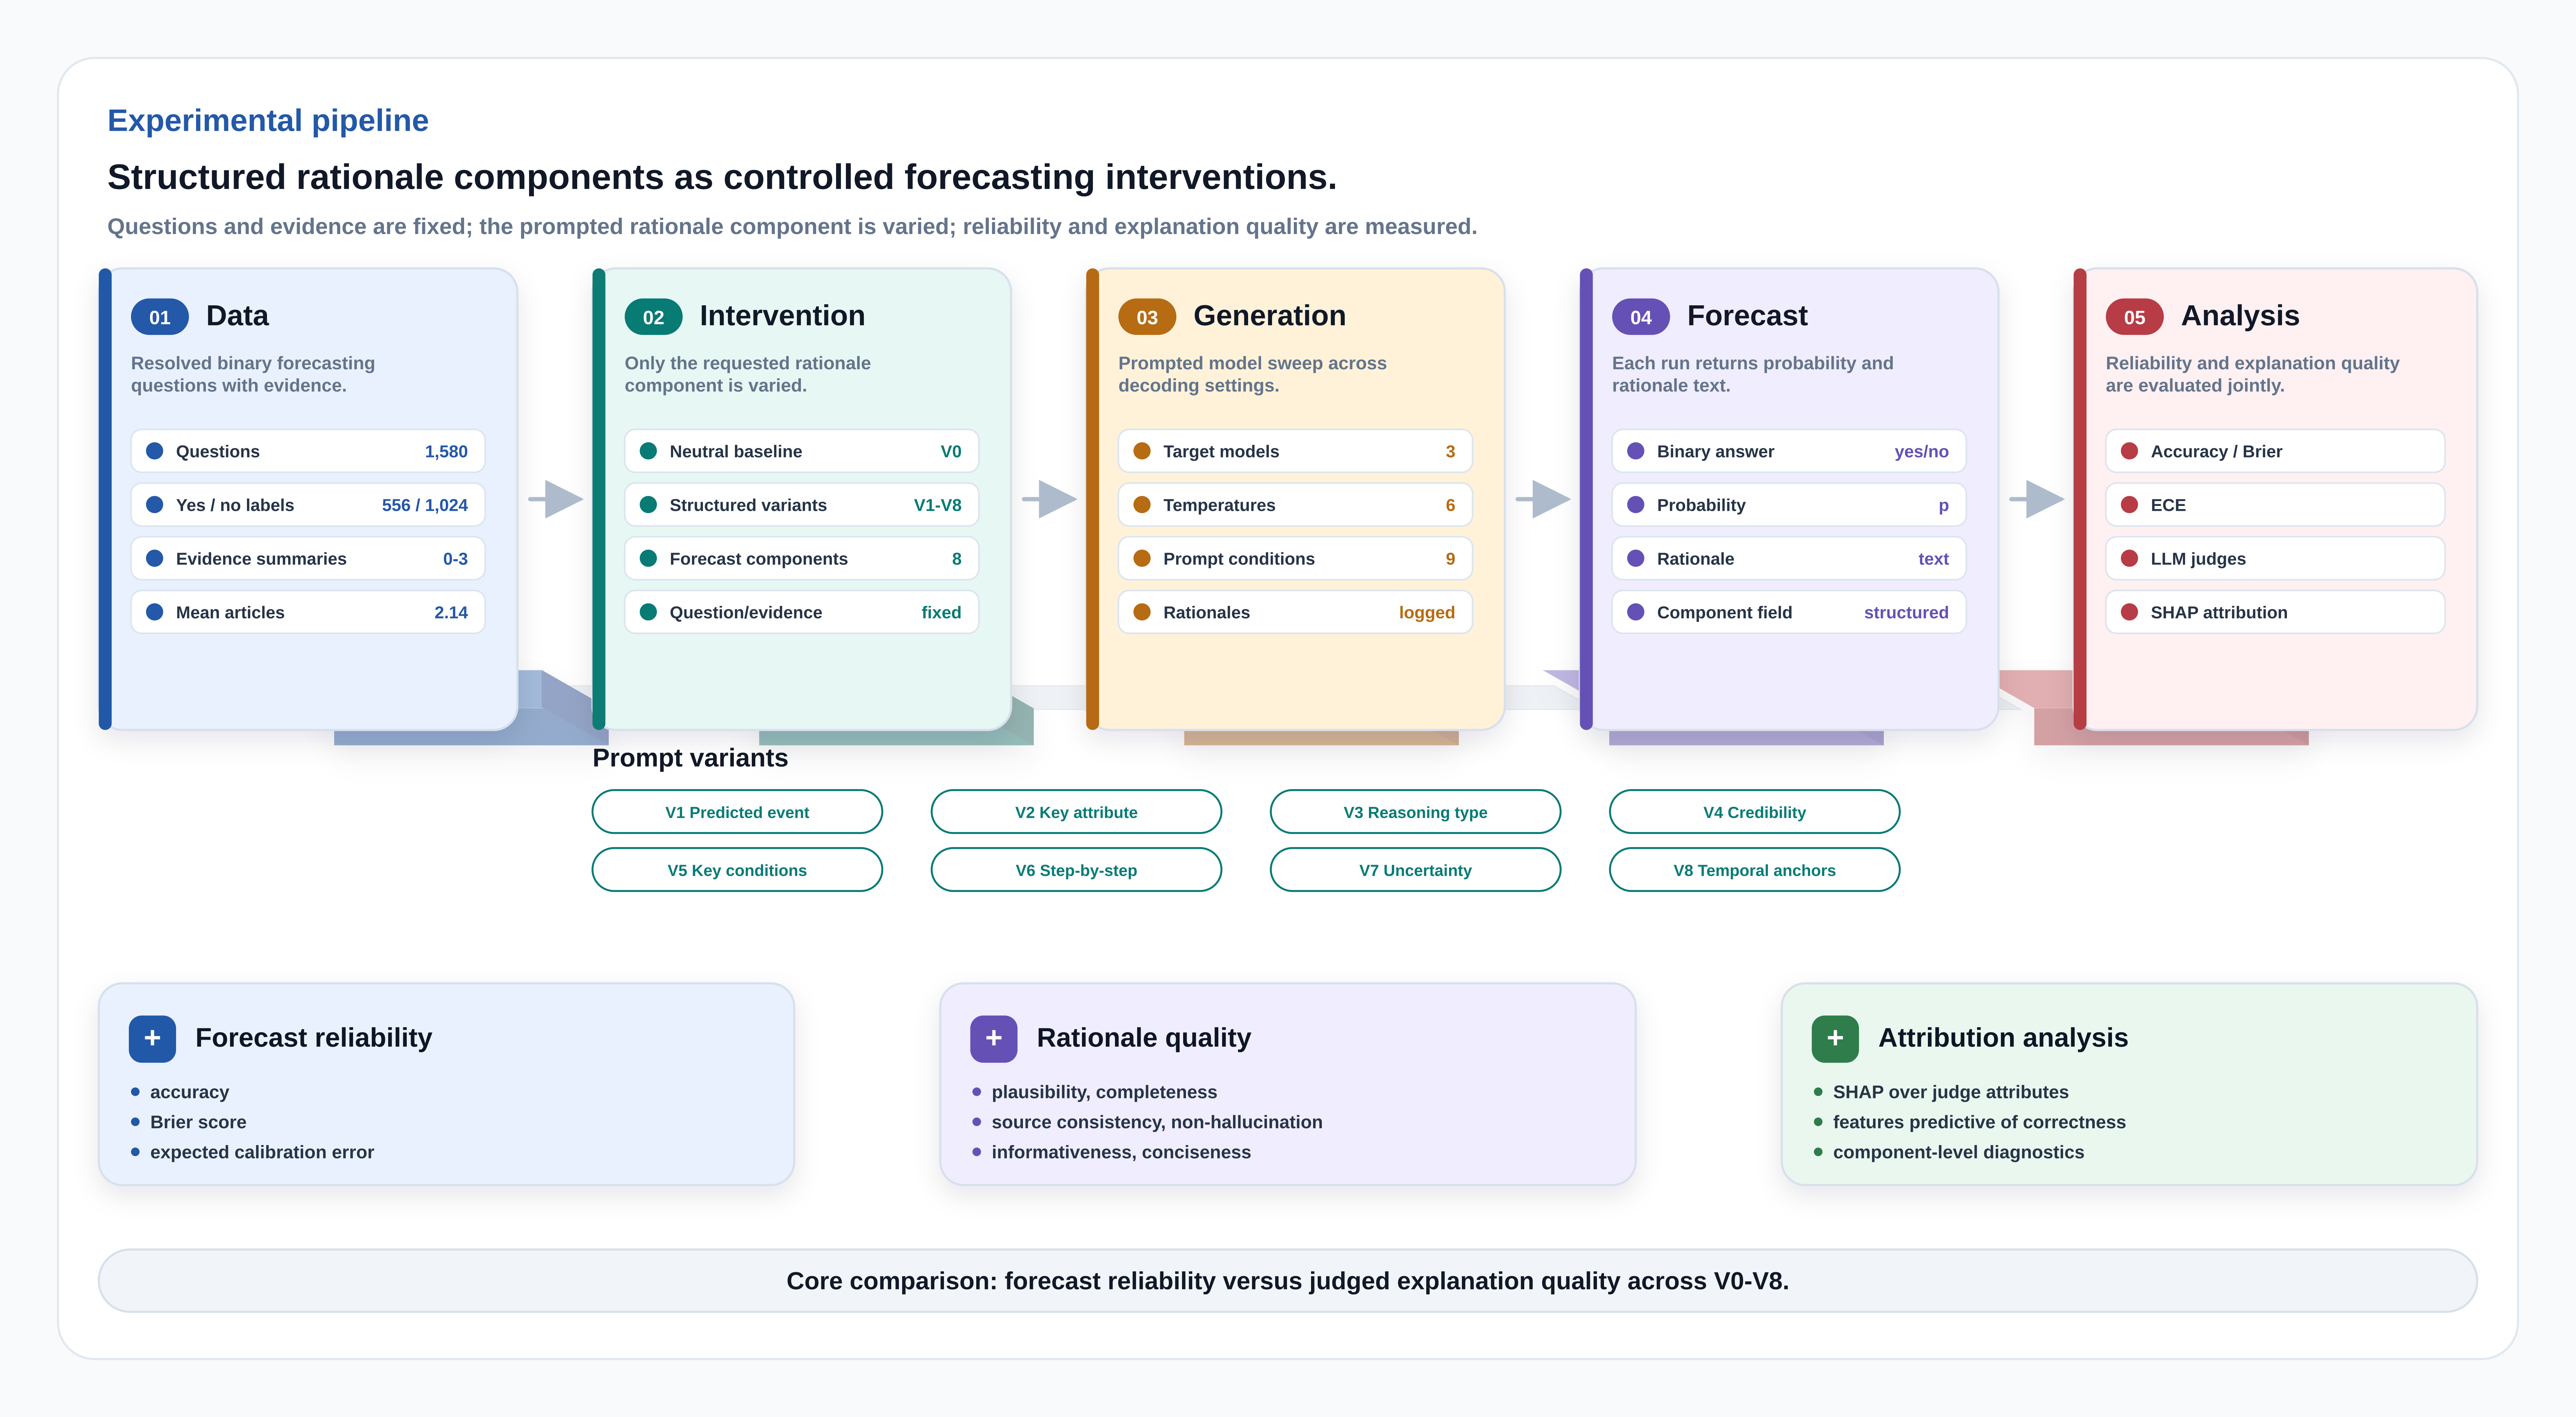
\includegraphics[width=\textwidth]{project_pipeline_acl_three.png}
    \caption{Experimental pipeline for evaluating structured rationale components in binary event forecasting.}
    \label{fig:pipeline}
\end{figure*}

\subsection{Dataset Construction}

We use the released dataset \texttt{forecasting\_qa\_news\_metaculus\_2025-02-01\_to\_today.metaculus\_frs\_format.json}.
It contains 1,580 resolved Metaculus-style binary questions with verified yes/no outcomes.
Of these questions, 556 resolve to \textsc{yes} and 1,024 resolve to \textsc{no}.
Each record contains the original question text, description, resolution criteria, category labels, creation and publication times, resolution time, days open, and a search query used to associate evidence.

Each question is paired with up to three evidence articles.
The article fields include URL, title, raw text, authors, publication date, extractive or LLM-generated summaries, keywords, Forecast Relevance Score (FRS), and a credibility score.
The average number of associated evidence articles is 2.14.
We verified that article timestamps in the current dataset precede the corresponding resolution timestamp, so the evidence supplied to the model is pre-resolution evidence.
Because the experiment conditions on provided evidence, the task is best understood as evidence-conditioned forecasting rather than purely parametric prediction from a model's pretraining data.

\subsection{Prompt Variants}

All runs use a shared system instruction that restricts the model to the provided question, description, resolution criteria, and evidence summaries.
The model must output valid JSON with \texttt{predicted\_answer}, \texttt{confidence}, and \texttt{rationale}.
Structured variants either add a required field or impose a targeted constraint on the rationale.
Table~\ref{tab:variants} lists the nine prompt conditions.
Unlike earlier pilot drafts, V4 is part of the evaluated sweep: it asks the model to ground the rationale in source credibility, evidence quality, and recency.

\begin{table}[t]
\centering
\small
\begin{tabular}{ll}
\toprule
Variant & Prompt intervention \\
\midrule
V0 & Neutral baseline \\
V1 & State the concrete predicted event \\
V2 & Identify the key attribute: time, quantity, or actor \\
V3 & Declare reasoning type: speculation, plan, expert forecast, trend \\
V4 & Discuss evidence credibility, quality, and recency \\
V5 & List two to four key conditions \\
V6 & Provide two to three numbered reasoning steps \\
V7 & Use explicit uncertainty language \\
V8 & Mention relevant dates or time ranges \\
\bottomrule
\end{tabular}
\caption{Prompt variants used in the forecasting sweep.}
\label{tab:variants}
\end{table}

\subsection{Models and Inference}

The complete quantitative sweep reported in this paper covers three target models: Qwen2.5-7B-Instruct, Qwen3-32B, and GPT-OSS-120B.
The repository also contains configuration entries and partial artifacts for additional hosted models, but we restrict the main analysis to models with complete metric tables.
For each target model, we evaluate all nine prompt variants at six nominal temperatures:
\[
T \in \{0.0, 0.25, 0.75, 1.25, 1.75, 2.0\}.
\]
Temperature directory names differ slightly across providers, but the analysis scripts normalize them when aggregating results.

Inference is config-driven through \texttt{configs/models.yaml} and \texttt{configs/variants.yaml}.
Each run writes JSON outputs and metadata including provider, resolved model identifier, temperature, output schema, and prompt hashes.
The pipeline supports sharded execution, retrying null or malformed outputs, resuming incomplete runs, dataset validation, and result verification.
Malformed predictions and missing rows are not silently dropped: they are counted as missing outputs in the metric summaries.

\subsection{Forecast Evaluation}

Let $y \in \{0,1\}$ denote the resolved answer and let $\hat{a}$ be the model's predicted yes/no label with confidence $c \in [0,1]$.
We convert the output to a probability of \textsc{yes} as follows:
\[
\yesprob =
\begin{cases}
c, & \hat{a}=\textsc{yes},\\
1-c, & \hat{a}=\textsc{no}.
\end{cases}
\]
We report accuracy, Brier score \cite{brier1950verification}, and expected calibration error (ECE) \cite{guo2017calibration}.
Accuracy evaluates the binary label.
Brier score evaluates probabilistic error using $\frac{1}{N}\sum_i(\yesprob_i-y_i)^2$.
ECE is computed with 10 equal-width confidence bins and compares predicted-label confidence to empirical correctness within each bin.

\subsection{Automatic Rationale Evaluation}

We evaluate rationale quality with two automatic LLM judges: Gemma-4-31B-it and Kimi-K2.5.
For each question, the judge receives the shared forecasting context and evidence digest, along with the rationales produced by the prompt variants.
Judges are explicitly instructed not to score forecast correctness; correctness is computed separately from the resolved labels.
Each judge assigns six scores on a 0--1 scale: plausibility, completeness, source consistency, non-hallucination, informativeness, and conciseness.
We report per-attribute scores and their mean as an overall rationale-quality score.

\subsection{Diagnostic Attribution}

Finally, we ask whether judged rationale attributes are predictive of forecast correctness.
We fit a classifier using the six judged rationale attributes as input features and forecast correctness as the target, then compute SHAP feature importances.
This analysis is diagnostic rather than causal: it identifies which judged properties co-vary with correct forecasts, but it does not prove that those properties caused the model's prediction.

\section{Results}

\subsection{Temperature Effects}

Table~\ref{tab:temperature} reports the best temperature per model by mean Brier score, averaging over all prompt variants.
The strongest model in the current sweep is GPT-OSS-120B, while both Qwen models perform best at deterministic decoding.

\begin{table}[t]
\centering
\small
\begin{tabular}{lrrrr}
\toprule
Model & Temp. & Acc. & Brier & ECE \\
\midrule
GPT-OSS-120B & 0.25 & 0.817 & 0.166 & 0.121 \\
Qwen2.5-7B-Instruct & 0.00 & 0.734 & 0.200 & 0.112 \\
Qwen3-32B & 0.00 & 0.712 & 0.214 & 0.112 \\
\bottomrule
\end{tabular}
\caption{Best temperature per model by mean Brier score across variants.}
\label{tab:temperature}
\end{table}

\subsection{Prompt Variant Effects}

Table~\ref{tab:variant-best} compares the neutral baseline to the best observed structured variant for each model under different metrics.
The effect of structure is model-dependent.
GPT-OSS-120B benefits most from temporal anchors, which improve mean Brier score from 0.164 to 0.162.
Qwen3-32B obtains its best accuracy and ECE under credibility framing, but this does not improve Brier score.
Qwen2.5-7B-Instruct is strongest under the neutral baseline for accuracy and Brier score, although reasoning-type prompts slightly improve ECE.

\begin{table*}[t]
\centering
\small
\begin{tabular}{llrrr}
\toprule
Model & Condition & Acc. & Brier & ECE \\
\midrule
\multirow{4}{*}{GPT-OSS-120B}
& Baseline & 0.815 & 0.164 & 0.104 \\
& Best Brier: V8 temporal anchors & 0.817 & 0.162 & 0.103 \\
& Best ECE: V5 key conditions & 0.809 & 0.164 & 0.098 \\
& Best accuracy: V8 temporal anchors & 0.817 & 0.162 & 0.103 \\
\midrule
\multirow{4}{*}{Qwen2.5-7B}
& Baseline & 0.743 & 0.196 & 0.104 \\
& Best Brier: V0 baseline & 0.743 & 0.196 & 0.104 \\
& Best ECE: V3 reasoning type & 0.725 & 0.201 & 0.098 \\
& Best accuracy: V0 baseline & 0.743 & 0.196 & 0.104 \\
\midrule
\multirow{4}{*}{Qwen3-32B}
& Baseline & 0.715 & 0.208 & 0.106 \\
& Best Brier: V0 baseline & 0.715 & 0.208 & 0.106 \\
& Best ECE: V4 credibility & 0.730 & 0.211 & 0.086 \\
& Best accuracy: V4 credibility & 0.730 & 0.211 & 0.086 \\
\bottomrule
\end{tabular}
\caption{Prompt-variant effects averaged over temperature runs. Lower Brier and ECE are better.}
\label{tab:variant-best}
\end{table*}

Aggregating across the three models, the neutral baseline has the best mean Brier score (0.189), followed by temporal anchors (0.193) and credibility framing (0.195).
This aggregate result should not be over-interpreted because model-specific effects are heterogeneous.
It does, however, show that adding an explicit rationale component can impose costs as well as benefits.

\subsection{Rationale Quality}

Automatic judge scores do not simply reward longer or more structured outputs.
In the currently available judged runs, the neutral baseline often receives the highest overall judge score, especially for GPT-OSS-120B and both Qwen models.
Step-by-step reasoning and uncertainty-language prompts are usually competitive but do not dominate.
This suggests that concise free-form rationales can be judged as more plausible or source-consistent than forced schemas when the schema encourages formulaic text.

\subsection{Predicting Correctness from Rationale Attributes}

The SHAP analysis in Table~\ref{tab:shap} links automatic rationale attributes to forecast correctness.
The rationale-evaluation sample contains 42,660 model--variant--question rows when missing rationales are included; using the 42,652 rows with complete combined mean judge scores, the attribute classifier obtains ROC-AUC 0.726 and accuracy 0.646.
Completeness and plausibility are the strongest features by mean absolute SHAP value.
Informativeness, non-hallucination, and source consistency differ between correct and incorrect forecasts but have lower attribution magnitude in the fitted model.

\begin{table}[t]
\centering
\small
\begin{tabular}{lrrr}
\toprule
Feature & Mean & Correct--Incorrect & Mean $|\mathrm{SHAP}|$ \\
\midrule
Completeness & 0.742 & 0.138 & 0.074 \\
Plausibility & 0.792 & 0.128 & 0.060 \\
Informativeness & 0.740 & 0.119 & 0.027 \\
Non-hallucination & 0.686 & 0.117 & 0.024 \\
Conciseness & 0.911 & 0.024 & 0.019 \\
Source consistency & 0.719 & 0.134 & 0.011 \\
\bottomrule
\end{tabular}
\caption{Rationale-attribute feature importance for predicting forecast correctness using combined judge scores.}
\label{tab:shap}
\end{table}

\section{Discussion}

Our experiments show that rationale structure affects forecasting behavior, but its effects are heterogeneous across models and metrics.
The neutral baseline is a strong reference point: averaged over all temperatures, it remains best for Qwen2.5-7B and Qwen3-32B by Brier score, and it is competitive for GPT-OSS-120B.
This cautions against treating more structured rationales as automatically better forecasts.
Structured prompts are interventions on the model's reasoning format, and the same intervention can improve one metric while degrading another.

\subsection{Prompt Structure and Calibration}

The most useful structured variants are model dependent.
For GPT-OSS-120B, temporal anchors achieve the best average Brier score among variants, while key conditions give the lowest average ECE.
For Qwen2.5-7B, the neutral baseline performs best overall, with temporal anchors close behind; key conditions substantially reduce accuracy and worsen calibration.
For Qwen3-32B, credibility framing gives the highest accuracy and lowest ECE, while the neutral baseline gives the best Brier score.
Thus, temporal and evidential cues can be useful, but their benefits are not universal.

Explicit uncertainty language does not reliably improve calibration.
Across models, the uncertainty variant often changes the surface form of the rationale without producing better probability estimates.
This supports a distinction between verbal uncertainty and probabilistic calibration: hedging expressions such as ``likely'' or ``possible'' may make explanations appear more cautious, but they do not guarantee better numeric confidence.

\subsection{Temperature and Coverage}

Temperature effects are also model specific.
Using Brier score as the selection criterion, GPT-OSS-120B performs best at $T=0.25$, while Qwen2.5-7B and Qwen3-32B perform best at deterministic decoding.
GPT-OSS-120B is relatively stable for $T \leq 0.75$, whereas both Qwen models degrade as temperature increases.
High-temperature settings also introduce more missing or invalid generations, especially for GPT-OSS-120B at $T=2.0$ and Qwen3-32B at $T=2.0$.
For forecasting, temperature should therefore be tuned jointly with output validity, Brier score, and calibration rather than selected only for diversity.

\subsection{Forecasting Summaries}

The forecasting-summary component improves average performance, but not uniformly.
At $T=0$, adding summaries improves the average across the three evaluated models from 0.736 to 0.756 accuracy, from 0.205 to 0.193 Brier score, and from 0.131 to 0.116 ECE.
The gains are clearest for Qwen2.5-7B and Qwen3-32B, suggesting that structured evidence summaries help models use retrieved context more effectively.
GPT-OSS-120B is an exception: its accuracy is unchanged, and its Brier score and ECE are better without summaries in this ablation.
This indicates that stronger models may already extract enough signal from raw evidence, while smaller models benefit more from explicit forecasting-oriented summaries.

\subsection{Rationale Quality as a Diagnostic Signal}

The LLM-judge analysis shows that rationale quality tracks forecast correctness but is not identical to it.
Correct forecasts receive higher scores on all six judged attributes.
The largest raw gaps are for completeness, source consistency, and plausibility, indicating that correct forecasts tend to be more complete, better grounded in the supplied evidence, and more plausible.
In the multivariate SHAP analysis, completeness and plausibility are the strongest marginal predictors of correctness.
Source consistency has a large raw correctness gap but the lowest SHAP importance, suggesting that its signal overlaps with completeness, plausibility, and informativeness.
Conciseness contributes little in both analyses.

These results should be interpreted as correlational.
Judge scores are assigned after the forecast is generated, so they do not establish that improving a rationale attribute would causally improve the forecast.
Rather, they show that rationale attributes are useful diagnostic signals for identifying when a forecast is more likely to be correct.

\subsection{Implications}

The main implication is that rationale design should be evaluated with forecasting metrics, not only with explanation-quality judgments.
Structured rationales can expose evidence use and reasoning quality, but they can also harm calibration or reduce robustness.
For deployment, neutral and temporal-anchor prompts are sensible starting points, credibility framing should be considered for models that benefit from evidence filtering, and uncertainty-language prompts should not be treated as calibration methods.
Forecasting summaries are useful on average, especially for smaller models, but their value should be validated per model.

\section{Limitations}

This draft reports the complete metrics currently available in the repository: three target models, nine prompt variants, and six temperature settings.
The model configuration includes additional systems, but incomplete or partial runs should not be presented as final results until verified.
The rationale-quality evaluation is automatic rather than human-annotated, and LLM judges may share biases with the models being evaluated.
The dataset is drawn from Metaculus-style resolved questions with retrieved news evidence, so results may not generalize to domains where evidence is private, highly technical, or adversarial.
Finally, SHAP analysis is correlational and should not be interpreted as proving that making a rationale more plausible or complete will causally improve forecast accuracy.

\section{Ethical Considerations}

Forecasting systems can influence decisions in finance, policy, public health, and security.
Poorly calibrated forecasts or persuasive but unsupported rationales may mislead users.
Our framework is intended for evaluation and diagnostic use, not as evidence that LLM forecasts should be deployed without human oversight.
The dataset contains public forecasting questions and article-derived evidence, but future releases should document source licenses and remove any sensitive content that appears in retrieved articles.

\section{Extended Uncertainty Analysis}
\label{app:uncertainty}

This appendix compares natural uncertainty language in V0 with forced uncertainty language in V7 at $T=0.0$ using forecasting summaries.

\subsection{Uncertainty Expression Patterns}

We count lexical uncertainty markers in rationales using patterns for hedging terms, epistemic markers, and strong uncertainty expressions.
V7 substantially increases explicit uncertainty language, but this lexical shift does not improve calibration.

\begin{table}[h]
\centering
\small
\begin{tabular}{lcc}
\toprule
\textbf{Metric} & \textbf{V0} & \textbf{V7} \\
\midrule
Has any uncertainty & 69.0\% & 95.9\% \\
Mean hedging markers & 0.63 & 1.41 \\
Mean epistemic markers & 1.11 & 1.03 \\
Mean strong uncertainty & 0.05 & 0.24 \\
\bottomrule
\end{tabular}
\caption{Uncertainty expression frequency in V0 and V7 rationales, aggregated across Qwen2.5-7B-Instruct, Qwen3-32B, and GPT-OSS-120B at $T=0.0$.}
\label{tab:uncertainty-freq}
\end{table}

\subsection{Matched Calibration Comparison}

We compare V0 and V7 on the same 1,580 questions for each model.
Positive $\Delta$ Brier and $\Delta$ ECE indicate degradation under V7.

\begin{table}[h]
\centering
\small
\begin{tabular}{lrrrr}
\toprule
\textbf{Model} & \textbf{V0 Brier} & \textbf{V7 Brier} & $\boldsymbol{\Delta}$ \textbf{Brier} & $\boldsymbol{\Delta}$ \textbf{ECE} \\
\midrule
Qwen2.5-7B & 0.187 & 0.199 & +0.011 & +0.009 \\
Qwen3-32B & 0.200 & 0.223 & +0.024 & +0.012 \\
GPT-OSS-120B & 0.159 & 0.177 & +0.018 & +0.026 \\
\midrule
Average & 0.182 & 0.200 & +0.018 & +0.016 \\
\bottomrule
\end{tabular}
\caption{Matched calibration comparison between V0 and V7 at $T=0.0$.}
\label{tab:calibration-matched}
\end{table}

Forced uncertainty language worsens calibration for all three completed models.
Average accuracy also falls from 76.7\% under V0 to 75.3\% under V7.

\subsection{Confidence Shifts}

V7 lowers mean confidence for all three models, but the reduction is not well aligned with correctness.

\begin{table}[h]
\centering
\small
\begin{tabular}{lrrr}
\toprule
\textbf{Model} & \textbf{V0 Conf.} & \textbf{V7 Conf.} & $\boldsymbol{\Delta}$ \\
\midrule
Qwen2.5-7B & 0.852 & 0.839 & -0.013 \\
Qwen3-32B & 0.774 & 0.702 & -0.073 \\
GPT-OSS-120B & 0.710 & 0.680 & -0.029 \\
\midrule
Average & 0.779 & 0.740 & -0.038 \\
\bottomrule
\end{tabular}
\caption{Mean predicted-label confidence under V0 and V7 at $T=0.0$.}
\label{tab:confidence-shifts}
\end{table}

On questions where V0 was incorrect, V7 reduces confidence by 0.012 for Qwen2.5-7B, 0.047 for Qwen3-32B, and 0.010 for GPT-OSS-120B.
This suggests that V7 can reduce overconfidence on some errors, but the effect is outweighed by worse overall Brier score and ECE.

\subsection{Interpretation}

The uncertainty prompt mainly changes language, not forecast reliability.
V7 makes rationales sound more cautious and lowers confidence, yet it degrades accuracy, Brier score, and ECE in the completed $T=0.0$ sweep.
Uncertainty language should therefore be treated as an interpretability device, not as a calibration method.

\section{Extended Temperature Analysis}
\label{app:temperature}

This appendix summarizes temperature sensitivity for the completed with-summaries sweep over Qwen2.5-7B-Instruct, Qwen3-32B, and GPT-OSS-120B.
Each model is evaluated across nine prompt variants and six temperature settings.

\subsection{Aggregate Results}

\begin{table}[h]
\centering
\small
\begin{tabular}{lrrrr}
\toprule
\textbf{Temperature} & \textbf{Acc.} & \textbf{Brier} & \textbf{ECE} & \textbf{Missing} \\
\midrule
$T=0.00$ & \textbf{75.6\%} & \textbf{0.193} & 0.116 & 0 \\
$T=0.25$ & 75.2\% & 0.195 & 0.117 & 1 \\
$T=0.75$ & 75.2\% & 0.196 & 0.118 & 1 \\
$T=1.25$ & 74.8\% & 0.198 & 0.117 & 0 \\
$T=1.75$ & 74.0\% & 0.203 & 0.123 & 14 \\
$T=2.00$ & 73.0\% & 0.209 & \textbf{0.107} & 47 \\
\bottomrule
\end{tabular}
\caption{Aggregate temperature results averaged across three models and nine prompt variants. Missing counts are summed over all model--variant cells.}
\label{tab:temp-aggregate}
\end{table}

On aggregate, $T=0.0$ gives the best accuracy and Brier score.
The lower ECE at $T=2.0$ should not be treated as an improvement because it coincides with the largest missing-output count and worse accuracy and Brier score.

\subsection{Per-Model Optima}

\begin{table}[h]
\centering
\small
\begin{tabular}{lrrrr}
\toprule
\textbf{Model} & \textbf{Best $T$} & \textbf{Acc.} & \textbf{Brier} & \textbf{ECE} \\
\midrule
Qwen2.5-7B-Instruct & 0.00 & 73.4\% & 0.200 & 0.112 \\
Qwen3-32B & 0.00 & 71.2\% & 0.214 & 0.112 \\
GPT-OSS-120B & 0.25 & 81.7\% & 0.166 & 0.121 \\
\bottomrule
\end{tabular}
\caption{Best temperature per model by mean Brier score across prompt variants.}
\label{tab:temp-model-optima}
\end{table}

Both Qwen models perform best under deterministic decoding.
GPT-OSS-120B is strongest at $T=0.25$ by Brier score, although its low-temperature results are close.
High-temperature sampling is consistently harmful for accuracy and Brier score, especially at $T \geq 1.75$.

\subsection{Practical Implications}

Temperature should be tuned per model rather than assumed transferable.
For the completed sweep, deterministic decoding is the safest default for Qwen models, while GPT-OSS-120B can benefit slightly from low stochasticity.
Temperatures at or above $1.75$ should be avoided for forecasting because they increase missing outputs and degrade probabilistic accuracy.

\section{Future Directions}
\label{app:future_directions}

\paragraph{Adaptive Prompt Routing.}
Future work should test routing policies that select between the neutral baseline, temporal anchors, and credibility framing by model, question category, evidence density, and time-to-resolution.
The goal is not to find a universally best rationale format, but to identify when a specific prompt creates incremental accuracy or calibration gains.

\paragraph{Probability Post-Processing.}
Several prompts change accuracy and ECE in different directions, so future systems should test held-out calibration methods such as temperature scaling, isotonic regression, and confidence clipping.
These methods are practical because they can improve the reliability of probability estimates without changing the underlying model.

\paragraph{Evidence Summarization for Signal Extraction.}
Forecasting summaries help on average but not uniformly.
A useful next step is to optimize summaries for resolution-relevant signals: base rates, recent trend changes, deadline constraints, and disconfirming evidence.
This should be evaluated by whether summaries improve out-of-sample Brier score, not by whether they make rationales more fluent.

\paragraph{Event-Driven Updating.}
Many forecasting opportunities depend on reacting to new evidence before it is fully priced in.
Future work should evaluate whether models update probabilities coherently when new articles arrive, how quickly they incorporate new information, and whether update rationales correctly identify the evidence that moved the forecast.

\paragraph{Robustness Checks.}
Forecasting pipelines should be tested against stale articles, irrelevant evidence, duplicated sources, misleading snippets, and prompt-injection text in retrieved documents.
Reliable forecasting depends on avoiding false signals, so robustness should be measured by performance under realistic retrieval noise.

\section{Conclusion}

We introduced a reproducible evaluation framework for structured LLM rationales in binary forecasting.
Across 1,580 resolved questions, three target models, and nine prompt conditions, we find that rationale structure has heterogeneous effects on accuracy, calibration, and judged explanation quality.
Temporal anchors and credibility framing can help specific models and metrics, but neutral rationales remain strong baselines.
Automatic rationale attributes, especially completeness and plausibility, are predictive of forecast correctness, supporting their use as diagnostic signals.
Future work should add human annotation, expand the model set, and test whether adaptive prompting can select the right rationale structure for each question.

\section{Hypothesis Validation}
\label{app:hypothesis_validation}

\begin{table}[H]
\centering
\resizebox{\columnwidth}{!}{
\begin{tabular}{lccc}
\hline
Hypothesis & Status & Acc. & ECE \\
\hline
H1: Predicted Event        & Rejected  & 75.0\% & 0.109 \\
H2: Key Attribute          & Rejected  & 75.3\% & 0.123 \\
H3: Reasoning Type         & Rejected  & 74.8\% & 0.109 \\
H4: Credibility            & Partial   & 76.6\% & 0.112 \\
H5: Key Conditions         & Rejected  & 74.3\% & 0.120 \\
H6: Step-by-Step Reasoning & Rejected  & 75.5\% & 0.129 \\
H7: Uncertainty Language   & Rejected  & 75.3\% & 0.123 \\
H8: Temporal Anchors       & Partial   & 76.6\% & 0.113 \\
V0: Neutral Baseline       & Reference & 76.7\% & 0.108 \\
\hline
\end{tabular}}
\caption{Hypothesis validation summary at $T=0.0$ using forecasting summaries, averaged across Qwen2.5-7B-Instruct, Qwen3-32B, and GPT-OSS-120B.}
\label{tab:hypothesis_validation}
\end{table}

Overall, the neutral baseline remains the strongest aggregate condition at $T=0.0$, with the highest accuracy and lowest ECE.
We therefore reject H1, H2, H3, H5, H6, and H7: predicted-event restatement, key-attribute identification, reasoning-type declaration, key-condition enumeration, step-by-step reasoning, and uncertainty language do not improve aggregate forecasting performance over the baseline.
H4 is partially supported because credibility framing nearly matches baseline accuracy and gives Qwen3-32B its best accuracy and ECE, but it does not improve the aggregate ECE.
H8 is also partially supported because temporal anchors nearly match baseline accuracy and improve GPT-OSS-120B, but they do not beat the aggregate baseline calibration.

\bibliographystyle{acl_natbib}
\bibliography{references}

\end{document}
